\documentclass{article}

\usepackage{amsmath}
\usepackage{graphicx}
\usepackage[hidelinks]{hyperref}

\setlength{\parindent}{0pt}
\setlength{\parskip}{10pt}

\begin{document}

\section*{Calculate power response of a loudspeaker}

Calculate approximate power response of a loudspeaker using SPL response on a sphere around the loudspeaker. The SPL responses $H_{m,n}$ are measured on two orbits as shown in the figure below ($m=1$ for the vertical orbit, $m=2$ for the vertical orbit). There are $N$ equally spaced points on each orbit ($n = 1\ldots N$).

\centerline{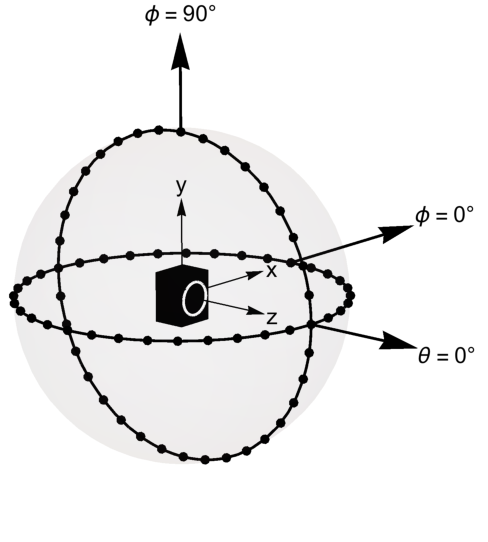
\includegraphics[width=0.3\linewidth]{orbits.pdf}}

The power response ($PR$) is the sound power summed over the sphere. If $w_n$ is the portion of the sphere surface covered by each point $(m,n)$, the summed power is:

\begin{equation*}
  PR = 10 \log_{10} \left( \sum_{m=1}^{2} \sum_{n=1}^{N} w_n |H_{m,n}|^2  \right) 
\end{equation*}

Note: $H_{m,n}$ is the SPL response at point $(m,n)$, in linear units (not dB).

Further reading: \url{https://www.princeton.edu/3D3A/Publications/Tylka_3D3A_DICalculation.pdf}
\end{document}


